\documentclass[10pt]{scrartcl}
\usepackage[latin1]{inputenc}
\usepackage[english, ngerman]{babel}
\usepackage[babel]{csquotes}
\usepackage{amsmath} % for eqref
\usepackage{tabularx}
\usepackage{pst-circ, pstricks-add}
\usepackage{graphicx}
\author{Denis Dietze \and Wolfgang Keller \and Nico Linke \and Thomas Schulte}

\title{Protokoll Einf\"uhrungsversuch E1}
\subtitle{Einsatz und Aufbau von Mess-- und Versorgungsger\"aten}
\begin{document}
\maketitle

\section{Studienkontrollfragen}

\subsection{Aufbau und Funktion von Drehspul-- und Dreheisenmesswerken}

\subsubsection{Drehspulmesswerke}

In einem \emph{Drehspulmesswerk} befindet ich im magnetischen Feld eines Dauermagneten\footnote{in modernen Ausf"uhrungen befindet sich der Dauermagnet h"aufig \emph{innerhalb} der Spule und nicht au"serhalb; unter anderem weil hierdurch St"orfelder abgeschirmt werden} eine drehbare Spule. Spiralfedern sind leitend mit der Spule verbunden und dienen sowohl der Stromversorgung als auch der R"ucksetzung in die Ruhelage.

Wird durch diese Spule Strom geleitet, so kommt es zur Wirkung der Lorentzkraft auf die Leiter der Spule. Diese dreht sich somit so weit, bis die Lorentzkraft gleich der winkelabh"angigen R"uckstellkraft der Feder ist (was einen Ausschlag des Zeigers, der mit der Spule verbunden ist, bewirkt). Da die Federkraft nach dem Hooke'schen Gesetz proportional zur Auslenkung ist, folgt eine lineare Einteilung der Skala.

\subsubsection{Dreheisenmesswerke}

In einem \emph{Dreheisenmesswerk} befindet sich innerhalb einer Spule mit feststehendem Weicheisenkern ein an Federn befestigter drehbarer Kern (ein so genanntes "`Dreheisen"'), welcher ebenfalls aus Weicheisen besteht. An diesem inneren Kern ist ein Zeiger befestigt.

Wenn Strom durch die Spule geleitet wird, so kommt es zur Magnetisierung beider Eisenkerne und der drehbare innere Kern dreht sich so weit, bis die Federkraft gleich der magnetischen Absto"sungskraft ist. Da diese Auslenkung nicht proportional zur Stromst"arke ist, ist die Skala im Allgemeinen nichtlinear.

\subsection{Messbereichserweiterung an Strom-- und Spannungsmessern}

\subsubsection{Messbereichserweiterung an Strommessern}

Um den Messbereich von Strommessern zu erweitern, schaltet man einen Widerstand \emph{parallel} zum Messwerk. Seien $R_M$ bzw. $R_P$ die Widerst"ande von Messger"at bzw. Shunt und $I_M$ bzw. $I_P$ die durch Messger"at bzw. Parallelwiderstand flie"senden Str"ome, sowie $I_{ges}=I_M+I_P$ der zu messende Strom.

Um den Messbereich n-fach zu erweitern, muss 
\begin{equation}
R_P=\frac{R_M}{n-1}
\label{eq:1}
\end{equation}
gew"ahlt werden, da gilt:

\begin{displaymath}
\frac{I_P}{I_M}=\frac{R_M}{R_P}.
\end{displaymath}

Wenn man hier Gleichung \eqref{eq:1} einsetzt, folgt:
\begin{equation}
\frac{I_P}{I_M}=n-1.
\label{eq:2}
\end{equation}

Unter Beachtung von
\begin{displaymath}
I_{ges}=I_M+I_P
\end{displaymath}
folgt somit aus Gleichung \eqref{eq:2}:
\begin{displaymath}
I_{ges}=n I_M,
\end{displaymath}
was einer n-fachen Messbereichserweiterung entspricht.

\subsubsection{Messbereichserweiterung an Spannungsmessern}

Um den Messbereich von Spannungsmessern auf das n-fache zu erweitern, schaltet man einen Widerstand von $R_R=(n-1) R_M$ \emph{in Reihe} mit dem Spannungsmessger"at, wobei $R_M$ bzw. $R_R$ den Widerstand des Spannungsmmessger"ats  bzw. in Reihe geschalteten Widerstands bezeichne. Stehe $U_M$ f"ur die am Spannungsmesser anliegende Spannung und $U_M$ f"ur die Summe der an Widerstand und Messger"at anliegenden Spannungen.

Mittels einer analogen Herleitung wie f"ur die Messbereichserweiterung f"ur Strommessger"ate kann man zeigen, dass dann gilt:

\begin{displaymath}
U_{ges}=n U_M.
\end{displaymath}

\subsection{Stromrichtige vs. spannungsrichtige Messschaltung}

\subsubsection{Stromrichtige Messschaltung}

\begin{pspicture}%[showgrid=true]
(0, 0)(10,6)
    \pnode(1, 1){A}
    \pnode(1, 4){B}
    \pnode(3, 4){C}
    \pnode(7.5, 4){D}
    \pnode(7.5, 1){E}
    \pnode(3, 1){F}
    \battery(A)(B){$E$}
    \circledipole[labeloffset=0, tensionlabel=$U_A$](C)(D){A}
    \circledipole[labeloffset=0, tensionlabel=$E{=}U_A+U_{R_L}$, tensionlabeloffset=2.2](C)(F){V}
    \wire(B)(C)
    \resistor[tensionlabel=$U_{R_L}$, tensionlabeloffset=1.4](D)(E){$R_L$}
    \wire(E)(F)
    \wire(F)(A)
\end{pspicture}

\subsubsection{Spannungsrichtige Messschaltung}

\begin{pspicture}%[showgrid=true]
(0, 0)(9,6)
    \pnode(1, 1){A}
    \pnode(1, 4){B}
    \pnode(4, 4){C}
    \pnode(7.5, 4){D}
    \pnode(7.5, 1){E}
    \pnode(4, 1){F}
    \battery(A)(B){$E$}
    \circledipole[labeloffset=0, tensionlabel=$I_g{=}I_V+I_{R_L}$](B)(C){A}
    \circledipole[labeloffset=0, tensionlabel=$I_V$, tensionlabeloffset=1.4](C)(F){V}
    \wire(C)(D)
    \resistor[tensionlabel=$I_{R_L}$, tensionlabeloffset=1.4](D)(E){$R_L$}
    \wire(E)(F)
    \wire(F)(A)
\end{pspicture}

\subsubsection{Unterschiede zwischen stromrichtiger und spannungsrichtiger Messschaltung}

Bei der \emph{stromrichtigen Messschaltung} ist das Strommessger"at in Reihe mit dem Widerstand geschaltet, was zur Folge hat, dass der durch den Widerstand flie"sende Strom korrekt gemessen wird. Das Spannungsmessger"at befindet sich dagegen parallel zu einer Reihenschaltung aus Widerstand und Strommessger"at, mit der Folge dass als Spannung die Summe aus der am Strommessger"at anliegenden Spannung $U_A$ und der am Widerstand anliegenden Spannung $U_{R_L}$ gemessen wird, w"ahrend wir "`eigentlich"' nur $U_{R_L}$ messen wollten. Es wird also bei dieser Messung eine h"ohere  Spannung gemessen, als am Widerstand anliegt.

Bei der \emph{spannungsrichtigen Messschaltung} dagegen ist das Spannungsmessger"at parallel zum Widerstand geschaltet. Die am Widerstand anliegende Spannung wird also korrekt gemessen. Das Strommessger"at befindet sich dagegen in Reihe mit einer Parallelschaltung aus dem Widerstand und dem Spannungsmessger"at. In der Folge wird die Summe der Str"ome durch das Spannungsmessger"at $I_V$ und den Widerstand $I_{R_L}$ gemessen, w"ahrend wir gerne den Strom durch den Widerstand messen w"urden - es wird also ein h"oherer Strom gemessen als durch den Widerstand flie"st.

\subsection{Gesichtspunkte bei der Auswahl von Messger"aten}

\begin{itemize}
\item Gew"unschte Art der Messung (direkte Messung vs. indirekte (d. h. Messung anderer Gr"o"sen, aus denen sich die gew"unschte Gr"o"se berechnet werden kann))
\item Messbereich
\item Empfindlichkeit des Messger"ates
\item Tr"agheit des Messger"ats in Bezug auf schnelle zeitliche "Anderungen der Messgr"o"se (sofern Messung von schnellen �nderungen erw�nscht ist)
\end{itemize}

\subsection{Empfindlichkeit von Messger"aten}

Nach DIN 1319 versteht man unter der Empfindlichkeit eines Messger"ats die "`"Anderung des Wertes der Ausgangsgr"o"se eines Messger"ates  bezogen auf die sie verursachende "Anderung des Wertes der Eingangsgr"o"se"', also als Formel:
\begin{displaymath}
S = \frac{\Delta \alpha}{\Delta x},
\end{displaymath}
wobei $\alpha$ f"ur den Wert der Ausgangsgr"o"se des Messger"ats (z. B. Zeigerausschlag) und x f"ur den Wert der Eingangsgr"o"se steht.

\subsection{Fehlerarten bei Messungen}
\label{sec:fehlerarten}

Es gibt 2 Arten von Fehlern:
\begin{itemize}
\item Systemische Fehler
\item Zuf"allige Fehler
\end{itemize}

\emph{Systemische Fehler} sind Fehler, die (wenn sie identifiziert sind) nach Betrag und Vorzeichen quantifiziert werden k"onnen. Des weiteren sind sie reproduzierbar. Somit kann man, wenn sie erkannt und erfasst sind, die Messwerte um den entsprechenden Fehler korrigieren.

\emph{Zuf"allige Fehler} dagegen sind prinzipiell unvermeidbar. Sie k"onnen Betrag und Vorzeichen wechseln und sind nicht reproduzierbar. Sie behandelt man mit statistischen Methoden.

\subsection{Aufbau und Funktionsprinzip des Elektronenstrahloszilloskops}

Ein Elektronenstrahloszilloskop besteht aus einer Elektronenstrahlr"ohre, an die in x- und y-Richtung kapazitativ ein elektrisches Feld angelegt wird, welches zu einer Ablenkung des Elektronenstrahls f�hrt.

\begin{pspicture}%[showgrid=true]
(0, -0.5)(11,7)
    \pnode(2.8, 4){Y}
	\pnode(1.5, 4){Z}
    \pnode(1.5, 0){A}
    \pnode(3, 0){B}
    \pnode(3, 0.5){B'}
    
    \pnode(5, 0.5){C'}
    \pnode(5, 0){C}
    \pnode(6.5, 0){D}
    \pnode(6.5, 4){E}
    \pnode(5.2, 4){F}
    
    \pnode(4, 2.8){G}
    \pnode(4, 1.5){H}
    \pnode(9, 1.5){I}
    \pnode(9, 3){J}
    
    \pnode(4, 5.2){K}
    \pnode(4, 6.5){L}
    \pnode(9, 6.5){M}
    \pnode(9, 5){N}
    
    \pnode(8.5, 3){J'}
    \pnode(8.5, 5){N'}
    
    \wire(Y)(Z)
    \wire(Z)(A)
    \wire(A)(B)
    \psline(2.8, 3.3)(2.8, 4.7)
    
    \tension[labeloffset=-0.5](B')(C'){$x(t)$}
    
    \wire(C)(D)
    \wire(D)(E)
    \wire(E)(F)
    \psline(5.2, 3.3)(5.2, 4.7)
    
    \wire(G)(H)
    \wire(H)(I)
    \wire(I)(J)
    \psline(3.3, 2.8)(4.7, 2.8)
    
    \wire(K)(L)
    \wire(L)(M)
    \wire(M)(N)
    \psline(3.3, 5.2)(4.7, 5.2)
    
    \tension[labeloffset=-0.5](J')(N'){$y(t)$}
    
    \pscircle(4,4){2}
\end{pspicture}

Je nach Wunsch des Nutzers, kann man nur an eine (y-Achse) oder beide Achsen eine Spannung anlegen. Falls man nur an die y-Achse eine Spannung anlegt, so wird an die x-Achse standardm��ig automatisch eine s�gezahnf�rmige Spannung mit bekannter Frequenz angelegt, so dass es im Oszillogramm so aussieht, als w�rde man das Signal gegen die Zeit oszillographieren.

\subsection{Frequenzmessung mittels Lissajousfiguren}

Die Entstehung der Figuren ist im Abschnitt \ref{abschnitt:liss} beschrieben. Um eine Frequenz mittels Lissajousfiguren zu messen, legt man an eine der beiden Achsen des Oszillographen die zu messenden Frequenz an und an die andere eine Referenzfrequenz.

Anschlie"send "andert man die Referenzfrequenz so lange, bis auf dem Oszillographen eine Lissajous-Figur sichtbar wird, f"ur die man das Frequenzverh"altnis kennt und rechnet hieraus die Frequenz aus.

\subsection{Das Prinzip der Wheatstoneschen Messbr"ucke}

\begin{pspicture}%[showgrid=true]
(1, 0)(9,7)
    \pnode(2, 1){A}
    \pnode(4, 1){B}
    \pnode(6, 1){C}
    \pnode(8, 1){D}
    \pnode(8, 3){E}
    \pnode(5, 3){F}
    \pnode(2, 3){G}
    \pnode(2, 6){H}
    \pnode(5, 6){I}
    \pnode(8, 6){J}
    \wire(A)(B)
    \battery(B)(C){$U=5~V$}
    \wire(C)(D)
    \wire(D)(E)
    \resistor(E)(F){$R_3$}
    \resistor(F)(G){$R_2$}
    \wire(G)(A)
    \circledipole[labeloffset=0, tensionlabel=$U_{Br}$, tensionlabeloffset=1.5](F)(I){V}
    \wire(D)(J)
    \wire(G)(H)
    \resistor(I)(J){$R_x$}
    \resistor[variable](H)(I){$R_1$}
\end{pspicture}

In der Schaltung der Wheatstoneschen Messbr"ucke gilt, wenn keine Spannung am Spannungsmessger"at anliegt:
\begin{displaymath}
  R_1 R_3 = R_2 R_x.
\end{displaymath}

Umgestellt nach $R_x$ ergibt sich:
\begin{equation}
 R_x = \frac{R_1 R_3}{R_2}.
 \label{eq:wheaton}
\end{equation}

Nun zur Erkl"arung des Vorgehens: der Widerstand $R_1$ ist variabel, w"arend $R_x$ den zu messenden Widerstand darstellt. Wir "andern den Widerstand $R_1$ so lange ab, bis keine Spannung mehr durch das Voltmeter flie�t. Da die Widerst"ande $R_1$, $R_2$ und $R_3$ bekannt sind, k"onnen wir mittels Gleichung \eqref{eq:wheaton} den Wert des unbekannten Widerstands $R_x$ ausrechnen.

\section{Versuchsdurchf"uhrung}

\subsection{Bestimmung der Widerstandswerte am Schiebewiderstand}

\subsubsection{Ergebnisse der Messung in stromrichtiger Messschaltung}

Die Ergebnisse der Messungen in stromrichtiger Messschaltung sind in Tabelle \ref{table:1} dargestellt.

\begin{table}
\begin{minipage}[t]{\textwidth}
\begin{center}
\begin{tabular}{|crrr|}
\hline
    gew"ahlte Klemmen & U \footnote{\label{fn:gemessen}gemessen} & I \footref{fn:gemessen} & R \footnote{aus gemessenem U und I berechnet; Genauigkeit zwei Dezimalstellen}\\
\hline
    1-2 & 5,1~V & 0,527~A & $9,68~\Omega$\\
    2-3 & 8,2~V & 0,508~A & $16,14~\Omega$\\
    1-3 & 8,2~V & 0,314~A & $26,11~\Omega$\\
\hline
\end{tabular}
\end{center}
\end{minipage}
\caption{Messergebnisse der Messung in spannungsrichtiger Messschaltung}
\label{table:1}
\end{table}

\subsubsection{Ergebnisse der Messung in spannungsrichtiger Messschaltung}

Die Ergebnisse der Messungen in stromrichtiger Messschaltung sind in Tabelle \ref{table:2} dargestellt.

\begin{table}
\begin{minipage}[t]{\textwidth} 
\begin{center} 
\begin{tabular}{|crrr|}
\hline
    gew"ahlte Klemmen & U \footnote{\label{fn:gemessen}gemessen} & I \footref{fn:gemessen} & R \footnote{aus gemessenem U und I berechnet; Genauigkeit zwei Dezimalstellen}\\
\hline
    1-2 & 5~V & 0,527~A & $9,49~\Omega$\\
    2-3 & 8,1~V & 0,508~A & $15,95~\Omega$\\
    1-3 & 8,1~V & 0,317~A & $25,55~\Omega$\\
\hline
\end{tabular}
\end{center}
\end{minipage}
\caption{Messergebnisse der Messung in stromrichtiger Messschaltung}
\label{table:2}
\end{table}

\subsubsection{Messung mittels Widerstands-Messger"aten}

Die Ergebnisse der Messungen sind in den Tabellen \ref{table:3} bis \ref{table:5} aufgelistet.

\begin{table}
\begin{minipage}[t]{\textwidth}
\begin{center}
\begin{tabular}{|cr|}
\hline
    Gew"ahlte Klemmen & R %\footnote{\label{fn:gemessen}gemessen}
    \\
\hline
    1-2 & $10,8~\Omega$\\
    2-3 & $16,9~\Omega$\\
    1-3 & $27,5~\Omega$\\
\hline
\end{tabular}
\end{center}
\end{minipage}
\caption{Messergebnisse der direkten Widerstandsmessung mittels Digitalmultimeter VC 150}
\label{table:3}
\end{table}

\begin{table}
\begin{minipage}[t]{\textwidth}
\begin{center}
\begin{tabular}{|cr|}
\hline
    Gew"ahlte Klemmen & R %\footnote{\label{fn:gemessen}gemessen}
    \\
\hline
    1-2 & $10,6~\Omega$\\
    2-3 & $17,0~\Omega$\\
    1-3 & $27,4~\Omega$\\
\hline
\end{tabular}
\end{center}
\end{minipage}
\caption{Messergebnisse der direkten Widerstandsmessung mittels Digitalvoltmeter G-1002.500}
\label{table:4}
\end{table}

\begin{table}
\begin{minipage}[t]{\textwidth}
\begin{center}
\begin{tabular}{|cr|}
\hline
    Gew"ahlte Klemmen & R %\footnote{\label{fn:gemessen}gemessen}
    \\
\hline
    1-2 & $10.5~\Omega$\\
    2-3 & $17,2~\Omega$\\
    1-3 & $26,5~\Omega$\\
\hline
\end{tabular}
\end{center}
\end{minipage}
\caption{Messergebnisse der direkten Widerstandsmessung mittels Kleinme"sbr"ucke nach Wheatstone bei einer Speisespannung von 5~V}
\label{table:5}
\end{table}

\subsection{Vergleich der Messergebnisse}

Die gemessenen bzw. aus den Messgr"o"sen berechneten Widerst"ande sind in Tabelle \ref{table:6} abgetragen.

\begin{table}
\begin{minipage}[t]{\textwidth}
\begin{center}
\begin{tabularx}{\textwidth}{|Xrrrr|}
\hline
    Messger"at/--methode & $R_{1, 2}$  & $R_{2, 3}$ & $R_{1, 2}+R_{2, 3}$ & $R_{1, 3}$ \\
\hline
    Stromrichtige Messung & $9,68~\Omega$ & $16,14~\Omega$ &  $25,82~\Omega$ & $26,11~\Omega$ \\
    Spannungsrichtige Messung & $9,49~\Omega$ & $15,95~\Omega$ & $25,44~\Omega$ & $25,55~\Omega$ \\
    Direkte Widerstandmessung Digitalmultimeter VC 150 & $10,8~\Omega$ & $16,9~\Omega$ & $27,7~\Omega$ & $27,5~\Omega$ \\
    Direkte Widerstandsmessung Digitalvoltmeter G-1002.500 & $10,6~\Omega$ & $17,0~\Omega$ & $27,6~\Omega$ & $27,4~\Omega$ \\
    Direkte Widerstandsmessung Kleinme"sbr"ucke nach Wheatstone & $10,5~\Omega$ & $17,2~\Omega$ & $27,7~\Omega$ & $26,5~\Omega$ \\
    Mittelwert aus allen Messungen & $10,214~\Omega$ & $16,638~\Omega$ & $26,852~\Omega$ & $26.612~\Omega$ \\
\hline
\end{tabularx}
\end{center}
\end{minipage}
\caption{Vergleich der Messergebnisse der angewendeten Messmethoden zur Widerstandsmessung}
\label{table:6}
\end{table}

Der Unterschied zwischen strom- und spannungsrichtiger Messsung l�sst sich dadurch erkl"aren, dass bei stromrichtiger Messung die Spannung leicht zu hoch gemessen wird (was gemessen wird ist $U_A+U_{R_L}$, was wir jedoch messen wollen ist $U_{R_L}$) und bei spannungsrichtiger Messung der Strom leicht zu hoch gemessen wird (gemessen wird $I_V+I_{R_L}$, was wir jedoch messen wollen ist $I_{R_L}$). Somit wird die aus $U_{R_L}$ und $I_{R_L}$ abgeleitete Gr"o"se $R_L$ bei stromrichtiger Messung untersch"atzt, denn es gilt:
\begin{displaymath}
R_L = \frac{U_{R_L}}{I_{R_L}} < \frac{U_{R_L}+U_A}{I_{R_L}}.
\end{displaymath}

Analog wird bei der spannungsrichtichtiger Messung die aus $U_{R_L}$ und $I_{R_L}$ abgeleitete gr"o"se $R_L$ "ubersch"atzt, denn es gilt:
\begin{displaymath}
R_L = \frac{U_{R_L}}{I_{R_L}} > \frac{U_{R_L}}{I_{R_L}+I_V}.
\end{displaymath}

In der Tat zeigt der Vergleich der Messwerte von strom-- und spannungsrichtiger Messung, dass die aus den Messwerten berechneten Werte f"ur den Widerstand in der Tat, wie aus der Theorie zu erwarten ist, bei der stromrichtigen Messung Gr"o"ser als bei der spannungsrichtigen Messung sind.

Die sonstigen Unterschiede in den Messergebnissen vermuten wir aufgrund allgemeiner systemische Fehler (vgl. Abschnitt \ref{sec:fehlerarten}), darunter
\begin{itemize}
\item Ungenauigkeiten (auch durch Alterungseffekte) der Messger"ate
\item bei Digitalmessger"aten Vort"auschung einer Messpr"azision durch viele angegebene Dezimalstellen, welche �ber der tats�chlichen Genauigkeit des Messger"ats liegt
\item bei der Wheatstone'schen Messbr"ucke eventuell nicht ganz pr"azise Einstellung auf den Nullpunkt aufgrund der Handhabung des Messger�ts
\item Erw"armung der Leiter infolge des Stromflusses f"uhrt zu ver"anderten Widerstandswerten
\item einen (wenn auch ausgesprochen geringen) Beitrag zum Fehler liefert ebenfalls, dass wir die Ergebnisse von Berechnungen auf 2 Nachkommastellen rundeten
\end{itemize}

\subsection{Effektiv-- und Spitzenwermessung mittels verschiedener Messger"ate}

Die gemessenen Spannung sind in Tabelle \ref{table:7} abgetragen.

\begin{table}
\begin{minipage}[t]{\textwidth}
\begin{center}
\begin{tabular}{|lr|}
\hline
    Messger"at & gemessene Spannung U \\
\hline
     Analogmultimeter 2010 & 1,8~V \\
     Digitalmultimeter VC 150 & 1,84~V \\
     Millivoltmeter MV 21 & 1,8~V \\
     Oszilloskop HM 203-7 & 5~V bzw. 2,5~V\footnote{ersterer Wert entspricht dem tats"achlich abgelesenen Wert f"ur $\widehat{U}$ bzw. $U_{ss}$, letzterer entsteht durch Division des ersteren durch 2 und entspricht $U_s$}\\
\hline
\end{tabular}
\end{center}
\end{minipage}
\caption{Ermittelte Spannungswerte f"ur verschiedene Messger"ate bei $\widehat{U}=5~V$ und $f=1000~Hz$}
\label{table:7}
\end{table}

Das "`Analogmultimeter 2010"', das "`Digitalmultimeter VC 150"' und das "`Millivoltmeter MV 21"' stellen bei der Spannung den Effektivwert dar, w"ahrend auf dem Oszilloskop (in diesem Fall vom Typ "`HM 203-7"') der Spitzenwert abgelesen werden kann.

Der Zusammenhang zwischen Effektivwert und Spitzenwert bei einer Sinusspannung ist
\begin{displaymath}
U_{eff} = \frac{1}{\sqrt{2}} U_s.
\end{displaymath}

\subsection{Oszillogramm einer Rechtecks-- und Sinusspannung}

\begin{figure}
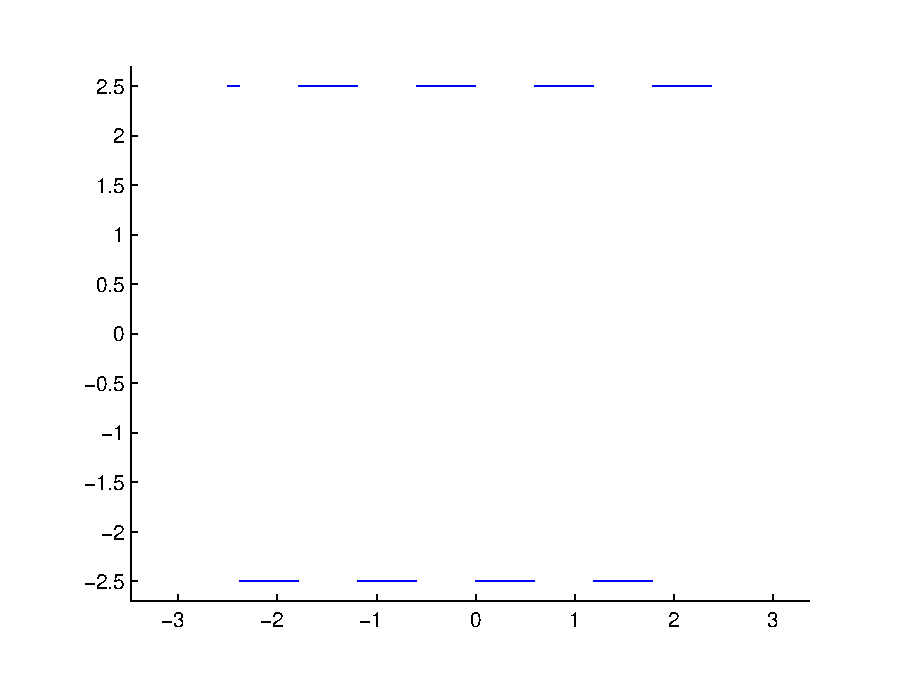
\includegraphics[width=0.5\textwidth]{rechteck_839hz.eps}
\caption{Oszillogramm einer Rechtecksspannung mit $2,5~V$ und $839~Hz$. Die Einheit der x-Achse ist $ms$ und die Einheit der y-Achse ist $V$.}
\label{fig:rechteck839}
\end{figure}

\begin{figure}
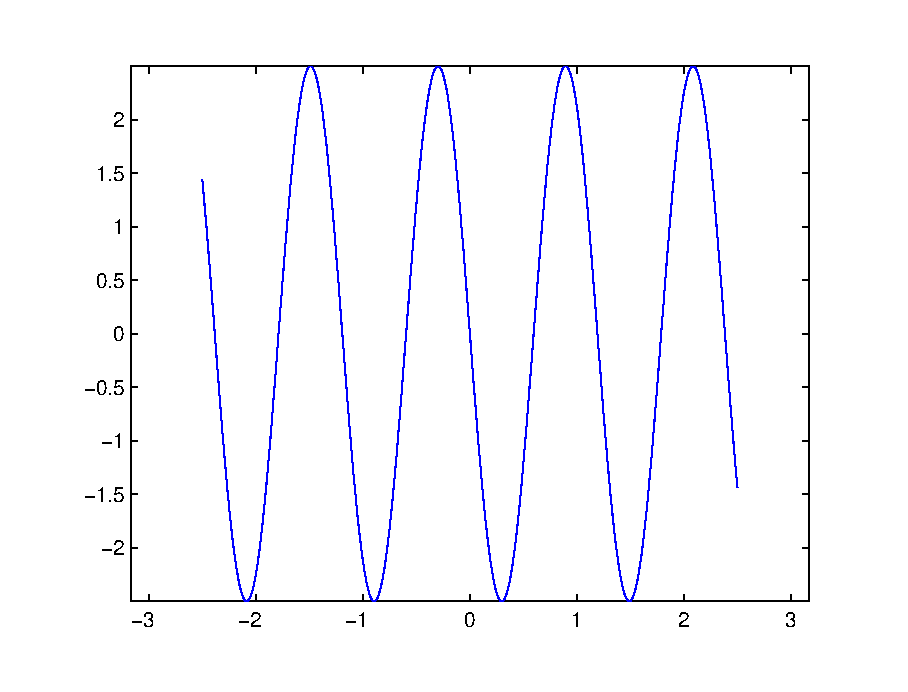
\includegraphics[width=0.5\textwidth]{sinus_839hz.eps}
\caption{Oszillogramm einer Sinus-Spannung mit Spitzenspannung $2,5~V$ und $839~Hz$. Die Einheit der x-Achse ist $ms$ und die Einheit der y-Achse ist $V$.}
\label{fig:sinus839}
\end{figure}

Die Oszillogramme bilden die Abbildungen \ref{fig:rechteck839} und \ref{fig:sinus839}. Um die Frequenz f�r die Sinusspannung abzulesen, misst man die Periodenl�nge (f�r Sinusspannungen geht dies sehr einfach �ber den Abstand zwischen einer geraden Anzahl an Nulldurchl"aufen der Kurve). F�r diese erh�lt man einen Wert von ca. $1,2~ms$, somit gilt f�r die Frequenz:
\begin{eqnarray*}
 f & = & \frac{1}{T} \\
  & = & \frac{1}{1,2~ms} \\
  & = & 833,3~Hz
\end{eqnarray*}

\subsection{Frequenzmessung mit Hilfe von Lissajous-Figuren}

\label{abschnitt:liss}

Die Frequenzverh"altnisse der Aufgabenstellung seien als $f_{y-Achse} : f_{x-Achse}$ zu betrachten. In den Abbildungen \ref{fig:0.5:1} bis \ref{fig:3:1} sind die in der Versuchsbeschreibung geforderten Skizzen der Lissajous-Figuren abgetragen. In allen diesen Abbildungen ist die an der x- und y-Achse verwendete Einheit "`Volt"'.

Die Figuren entstehen folgenderma"sen: an der x-- und y--Achse liegt je eine sinusf"urmige Spannung an:
\begin{eqnarray*}
u_x & = & U_s \sin (f_x 2 \pi t+\omega_x) \\
u_y & = & U_s \sin (f_y 2 \pi t+\omega_y),
\end{eqnarray*}
wobei $f_x, f_y$ f"ur die entsprechenden Frequenzen und $\omega_x, \omega_y$ f"ur die Phasenverschiebungen stehen. Da die Spitzenspannung an beiden Achsen im vorliegenden Experiment die selbe ist, wurde diese mit $U_s$ bezeichnet -- im Allgemeinen kann diese jedoch f"ur x- und y-Achse unterschiedlich sein.

Da die Auslenkung des Oszillographen proportional zur Spannung ist, erh"alt man somit die Gleichung der Lissajous-Figuren

\begin{displaymath}
\left(
\begin{array}{c}
u_x \\ u_y
\end{array} \right) = U_s
\left(
\begin{array}{c}
\sin (f_x 2 \pi t+\omega_x) \\ \sin (f_y 2 \pi t+\omega_y)
\end{array}
\right)
\end{displaymath}

f"ur $U_s=5~V$, Frequenzverh"altnisse nach Aufgabenstellung und in den Diagrammen angegebenen Werten f"ur $\omega_x$ und $\omega_y$ erh"alt die in den Abbildungen \ref{fig:0.5:1} bis \ref{fig:3:1} dargestellten Oszillogramme (bzw. mathematisch gesehen Trajektorien der angegebenen Kurvengleichung).

\begin{figure}
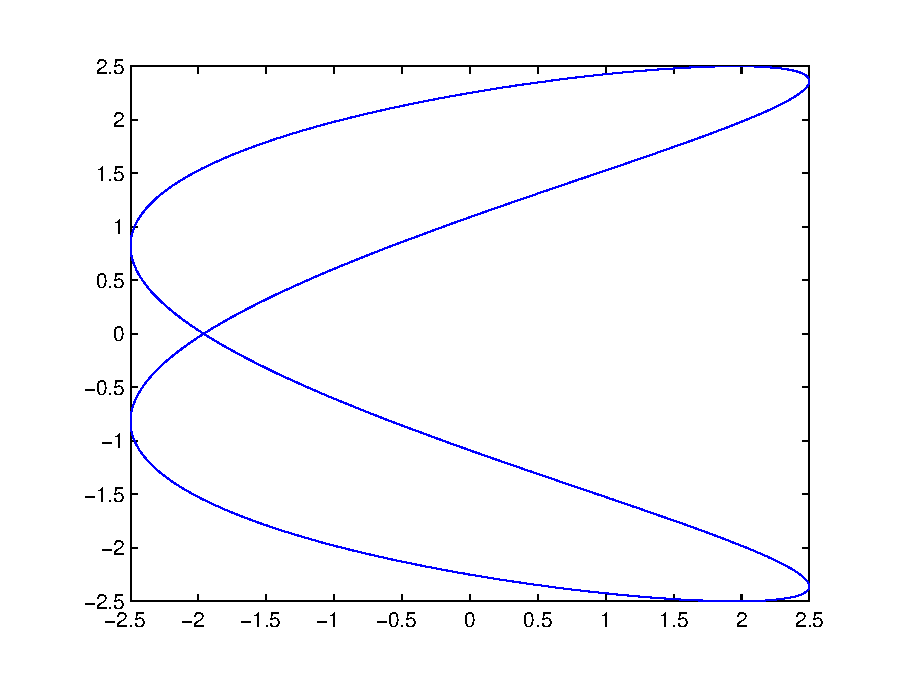
\includegraphics[width=0.5\textwidth]{05-1.eps}
\caption{Lissajous-Figur f"ur Frequenzverh"altnis 0,5:1, $\omega_x=0$ und $\omega_y=1,12$}
\label{fig:0.5:1}
\end{figure}

\begin{figure}
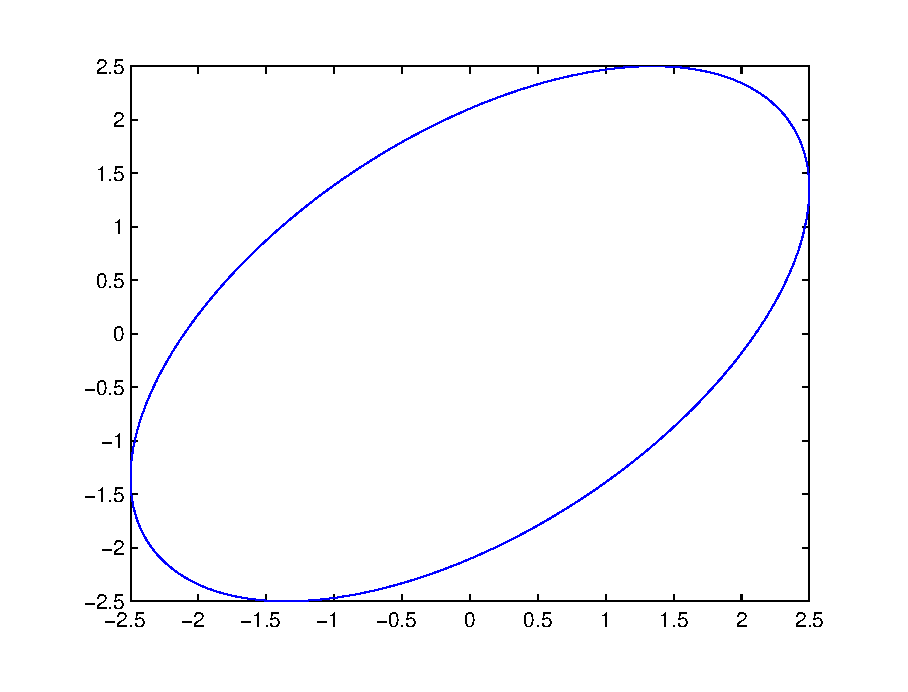
\includegraphics[width=0.5\textwidth]{1-1.eps}
\caption{Lissajous-Figur f"ur Frequenzverh"altnis 1:1, $\omega_x=0$ und $\omega_y=1$}
\label{fig:1:1}
\end{figure}

\begin{figure}
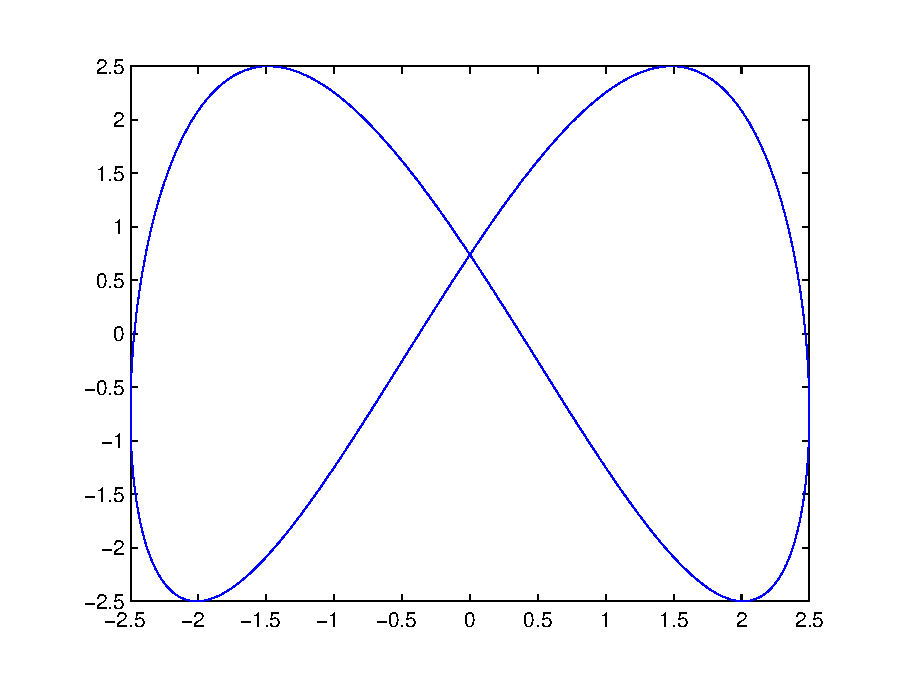
\includegraphics[width=0.5\textwidth]{2-1.eps}
\caption{Lissajous-Figur f"ur Frequenzverh"altnis 2:1, $\omega_x=0$ und $\omega_y=0,3$}
\label{fig:2:1}
\end{figure}

\begin{figure}
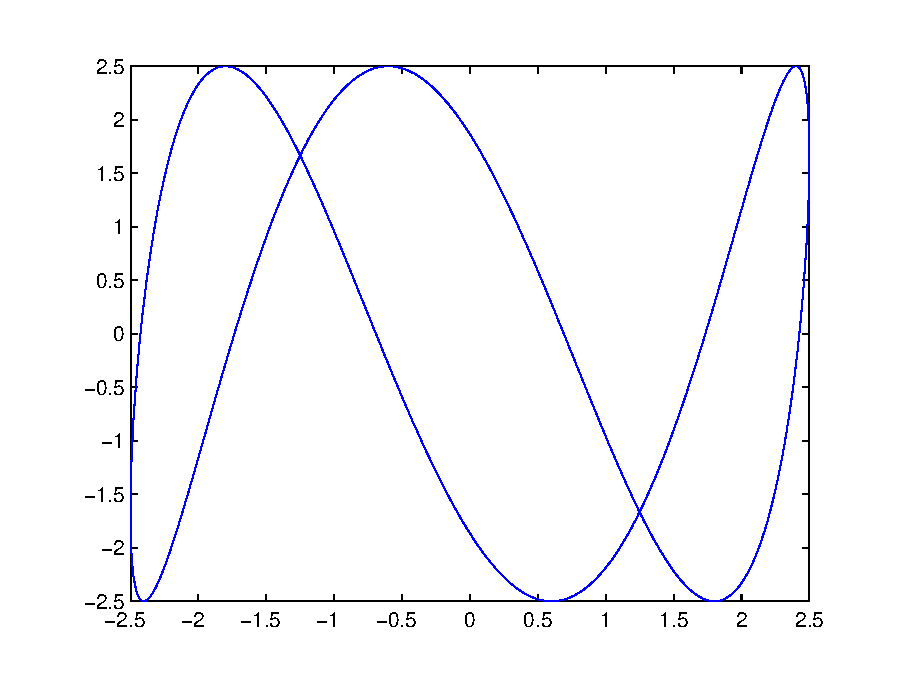
\includegraphics[width=0.5\textwidth]{3-1.eps}
\caption{Lissajous-Figur f"ur Frequenzverh"altnis 3:1, $\omega_x=0$ und $\omega_y=2,3$}
\label{fig:3:1}
\end{figure}

\end{document}